\begin{figure}[!ht]

\centering


\tikzset{every picture/.style={line width=0.75pt}} %set default line width to 0.75pt        

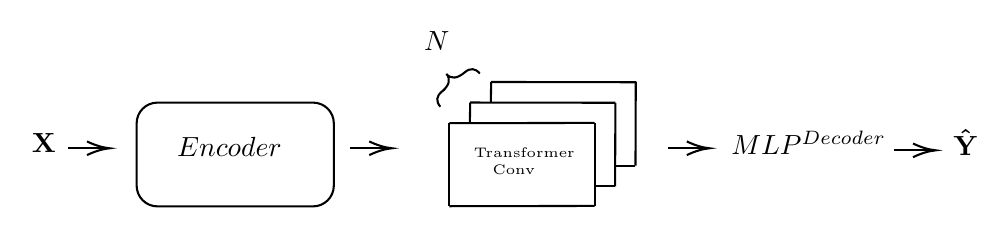
\begin{tikzpicture}[x=0.75pt,y=0.75pt,yscale=-1,xscale=1]
%uncomment if require: \path (0,300); %set diagram left start at 0, and has height of 300

%Shape: Brace [id:dp7019805664018027] 
\draw   (292.33,79) .. controls (290.14,76.39) and (287.74,76.19) .. (285.13,78.38) -- (285.13,78.38) .. controls (281.4,81.52) and (278.44,81.79) .. (276.25,79.18) .. controls (278.44,81.79) and (277.68,84.66) .. (273.95,87.79)(275.63,86.38) -- (273.95,87.79) .. controls (271.34,89.99) and (271.14,92.39) .. (273.33,95) ;
%Straight Lines [id:da24344825121139568] 
\draw    (277.63,102.92) -- (277.63,142.92) ;
%Straight Lines [id:da6110561454804792] 
\draw    (347.7,102.78) -- (347.7,142.78) ;
%Straight Lines [id:da03871795486024654] 
\draw    (277.63,102.92) -- (347.7,102.78) ;
%Straight Lines [id:da49608827752120055] 
\draw    (277.63,142.92) -- (347.7,142.78) ;
%Straight Lines [id:da27192408985546146] 
\draw    (287.69,92.96) -- (357.66,93.08) ;
%Straight Lines [id:da3480819733752343] 
\draw    (287.69,92.96) -- (287.55,102.87) ;
%Straight Lines [id:da3901687935554585] 
\draw    (297.79,83.06) -- (367.76,83.19) ;
%Straight Lines [id:da39197446094452226] 
\draw    (297.79,83.06) -- (297.66,92.98) ;
%Straight Lines [id:da01971233582821519] 
\draw    (357.52,133.35) -- (347.61,133.35) ;
%Straight Lines [id:da8552790800436195] 
\draw    (367.34,123.41) -- (357.43,123.41) ;
%Straight Lines [id:da901598531956911] 
\draw    (357.66,93.08) -- (357.52,133.35) ;
%Straight Lines [id:da7619590199519597] 
\draw    (367.48,83.15) -- (367.34,123.41) ;
%Straight Lines [id:da8643445648605664] 
\draw    (94,115) -- (112,115) ;
\draw [shift={(114,115)}, rotate = 180] [color={rgb, 255:red, 0; green, 0; blue, 0 }  ][line width=0.75]    (10.93,-3.29) .. controls (6.95,-1.4) and (3.31,-0.3) .. (0,0) .. controls (3.31,0.3) and (6.95,1.4) .. (10.93,3.29)   ;
%Straight Lines [id:da10221146771541123] 
\draw    (492,116) -- (510,116) ;
\draw [shift={(512,116)}, rotate = 180] [color={rgb, 255:red, 0; green, 0; blue, 0 }  ][line width=0.75]    (10.93,-3.29) .. controls (6.95,-1.4) and (3.31,-0.3) .. (0,0) .. controls (3.31,0.3) and (6.95,1.4) .. (10.93,3.29)   ;
%Straight Lines [id:da5913843902335524] 
\draw    (383,115) -- (401,115) ;
\draw [shift={(403,115)}, rotate = 180] [color={rgb, 255:red, 0; green, 0; blue, 0 }  ][line width=0.75]    (10.93,-3.29) .. controls (6.95,-1.4) and (3.31,-0.3) .. (0,0) .. controls (3.31,0.3) and (6.95,1.4) .. (10.93,3.29)   ;
%Rounded Rect [id:dp0019134800479860825] 
\draw   (127,103) .. controls (127,97.48) and (131.48,93) .. (137,93) -- (212,93) .. controls (217.52,93) and (222,97.48) .. (222,103) -- (222,133) .. controls (222,138.52) and (217.52,143) .. (212,143) -- (137,143) .. controls (131.48,143) and (127,138.52) .. (127,133) -- cycle ;
%Straight Lines [id:da4758105819320845] 
\draw    (230,115) -- (248,115) ;
\draw [shift={(250,115)}, rotate = 180] [color={rgb, 255:red, 0; green, 0; blue, 0 }  ][line width=0.75]    (10.93,-3.29) .. controls (6.95,-1.4) and (3.31,-0.3) .. (0,0) .. controls (3.31,0.3) and (6.95,1.4) .. (10.93,3.29)   ;

% Text Node
\draw (288,110) node [anchor=north west][inner sep=0.75pt]  [font=\tiny] [align=left] {\begin{minipage}[lt]{28.82pt}\setlength\topsep{0pt}
\begin{center}
{\tiny Transformer }\\{\tiny Conv}
\end{center}

\end{minipage}};
% Text Node
\draw (264,57.4) node [anchor=north west][inner sep=0.75pt]    {$N$};
% Text Node
\draw (412,105.4) node [anchor=north west][inner sep=0.75pt]    {$MLP^{Decoder}$};
% Text Node
\draw (75,106.4) node [anchor=north west][inner sep=0.75pt]    {$\mathbf{X}$};
% Text Node
\draw (519,104.4) node [anchor=north west][inner sep=0.75pt]    {$\mathbf{\hat{Y}}$};
% Text Node
\draw (145,108.4) node [anchor=north west][inner sep=0.75pt]    {$Encoder$};


\end{tikzpicture}


\caption{Architecture overview}
    \label{fig:architecture}
\end{figure}